%Empieza configuracion de capitulo
\setstretch{1.0}
\titleformat{\chapter}[block]{\Large\bfseries}{CHAPTER \Huge\thechapter\vspace{25 pt}}{0 pt}{\\\fontsize{26}{36}\selectfont}
\titlespacing{\chapter}{0 pt}{30 pt}{50 pt}[0 pt]
\titleformat{\section}{\Large\bfseries}{\thesection}{0 pt}{\hspace{30 pt}}
\titleformat{\subsection}{\large\bfseries}{\thesubsection}{0 pt}{\hspace{30 pt}}
\pagestyle{fancy}
\fancyhead[LO,LE]{\footnotesize\emph{\leftmark}}
\fancyhead[RO,RE]{\thepage}
\fancyfoot[CO,CE]{}
%Termina configuracion de capitulo

\chapter{Case Study: Detecting Conflicts on MexCom Use Cases} %Cambia al nombre de tu capitulo
\setstretch{1.5} %Regresa el interlineado a 1.5

\normalsize
\noindent
In this chapter, we verify the the use-cases studied in the previous chapter using our Promela model introduced in Chapter 3. The main purpose of this chapter is to prove the hypotheses introduced in chapter 1: \\
\begin{itemize}
\item \textbf{H1:} Rule-based Internet plans can be abstracted and specified in  a verification modeling language. 

\item \textbf{H2:} Model Checking can be used to verify whether the model meets the specification of the plan and to detect conflicts between the rules within the plans. 
\end{itemize}

In the sections below, each use-case is modeled and verified using our proposed Promela Model. 

\section{Core Rules}
\subsection{Promela Model}
\noindent
The model of the Core Rules and unlimited bolt-ons is shown in Listing \ref{CoreRules_Listing}. Given that a plan could consist of one or more rule instances, the worst case scenario was modeled; that is, one instance of each rule was selected to form the plan below.  \\

\singlespacing
\begin{lstlisting}[caption=Core-Rules-based Plan Model,
  label=CoreRules_Listing]
   // CoreRule
   Rules[0].conditions.application = 255;
   Rules[0].conditions.location = 255;
   Rules[0].action.underquota = 1; //Allow Traffic
   Rules[0].action.overquota = 0; //Block Traffic
   Rules[0].p = 0; 
   
   // Unlimited local Facebook Bolt-on
   Rules[1].conditions.application = 0;
   Rules[1].conditions.location = 0;
   Rules[1].action.underquota = 1; //Allow Traffic
   Rules[1].action.overquota = 1; //Allow Traffic
   Rules[1].p = 1;

   // Unlimited local Twitter Bolt-on
   Rules[2].conditions.application = 1;
   Rules[2].conditions.location = 0;
   Rules[2].action.underquota = 1; //Allow Traffic
   Rules[2].action.overquota = 1; //Allow Traffic
   Rules[2].p = 1;

   // Unlimited local Whatsapp Bolt-on
   Rules[3].conditions.application = 2;
   Rules[3].conditions.location = 0;
   Rules[3].action.underquota = 1; //Allow Traffic
   Rules[3].action.overquota = 1; //Allow Traffic
   Rules[3].p = 1;
\end{lstlisting}
\doublespacing

   
\subsection{System Properties}
\noindent The key rule of this plan, is the Rule[0] above; it dictates how most of the traffic should be handled. Basically, we are specifying no condition for that rule and indicating to apply the block action when the quota is reached. Please note that the amount of bytes of the quota of the Rule[0] is irrelevant as it is assumed that eventually the quota will be consumed regardless of the quota allowance. \\

Additionally there are three more rules, each one to always allow a different application. As it has been discussed, these additional rules shall have a higher priority, so the action to allow these particular applications (i.e.  facebook, twitter and whatsapp), takes precedence over the Rule[0].\\

If any of the additional rules has a lower priority assigned, the Rule[0] will take precedence over that rule and consequently, the desired behavior of allowing that particular application will not be met. \\

\begin{figure}[H]
\centering
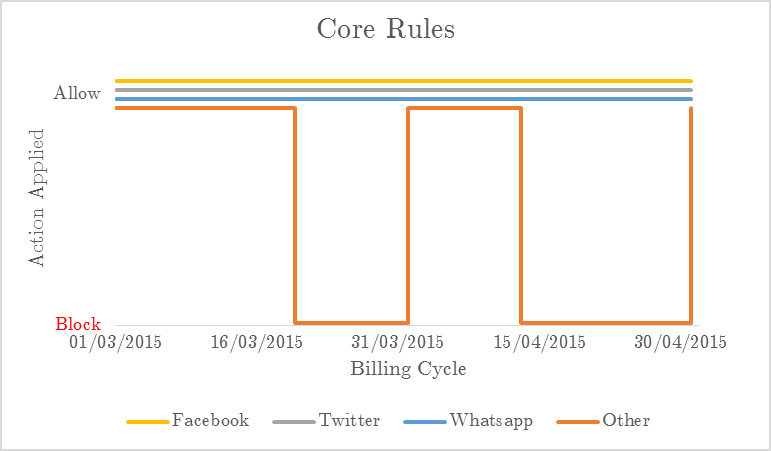
\includegraphics[width=1.00\textwidth]{image/Plans_CoreRules}
\caption{Core Rules - Linear Temporal Logic}
\label{coreRules}
\end{figure}

Figure \ref{coreRules} above, represent the expected behavior of this rule-based plan. Facebook, Twitter and Whatapp traffic shall always be allowed; while the rest of the traffic will be allowed and then eventually be blocked.  \\

In order to verify the expected behavior expressed above, the LTL below will be used. As seen in chapter 3, Linear-Temporal-Logic formulas are used to prove the property desired. 

\singlespacing
\begin{lstlisting}[caption=Core-Rules LTL,
  label=CoreLTL]
  ltl Core_Rules_LTL {
    []( 
        ((generated_rule_0 -> allowed_rule_0) -> <>blocked_rule_0) &&
    	(generated_rule_1->allowed_rule_1) &&
        (generated_rule_2->allowed_rule_2) &&
        (generated_rule_3->allowed_rule_3) 
      )
  }
\end{lstlisting}
\doublespacing

Listing \ref{CoreLTL} above can be translated to natural language as \emph{every} time traffic that meets the conditions of rules number 1, 2 and 3 is generated, then it will be allowed. Additionally, \emph{every} time traffic that meets the condition of rule number 0 is generated, then it will be allowed and \emph{eventually} will be blocked.

\subsection{SPIN Verification}
\noindent 
At this point we have intuitively specified the first rule-based plan with our Promela model and we have determined which LTL formulas will be used to verify the model. Listing \ref{CoreResult} below, presents the result obtained in Spin, with 0 errors shown in line 7.

\singlespacing
\begin{lstlisting}[caption=Core-Rules Plan Verification,
  label=CoreResult]
(Spin Version 6.3.2 -- 17 May 2014) + Partial Order Reduction
Full statespace search for:
	never claim         	+ (Core_Rules_LTL)
	assertion violations	+ (if within scope of claim)
	acceptance   cycles 	+ (fairness enabled)
	invalid end states	- (disabled by never claim)
State-vector 324 byte, depth reached 55, *** errors: 0 ***
       60 states, stored
       19 states, matched
       79 transitions (= stored+matched)
       48 atomic steps
hash conflicts:         0 (resolved)
Stats on memory usage (in Megabytes):
    0.019	equivalent memory usage for states (stored*(State-vector + overhead))
    0.143	actual memory usage for states
   64.000	memory used for hash table (-w24)
    0.069	memory used for DFS stack (-m2000)
   64.195	total actual memory usage
\end{lstlisting}
\doublespacing

\subsubsection{Exceptions Verification}
\noindent Our first results were expected, as the right priorities were assigned to each rule. For the next test, the priority of the key rule will be increased from 0 to 2, as shown below:

\singlespacing
\begin{lstlisting}[caption=Increased priority of the Core Rule,
  label=CoreRules_wrong]
   // CoreRule
   Rules[0].conditions.application = 255;
   Rules[0].conditions.location = 255;
   Rules[0].action.underquota = 1; //Allow Traffic
   Rules[0].action.overquota = 0; //Block Traffic
   Rules[0].p = 2; 
   ...
\end{lstlisting}
\doublespacing \bigskip

The updated model above, will not meet the LTL specification. The rules number 1, 2 and 3 will not be executed, because facebook, whatsapp and twitter traffic will be handled by the rule 0, which has a higher priority assigned. SPIN model basically identifies that when facebook traffic is generated, it is not always allowed.

\singlespacing
\begin{lstlisting}[caption=Invalid Core-Rules Plan - Verification ,
  label=InvalidCoreResult]
(Spin Version 6.3.2 -- 17 May 2014) + Partial Order Reduction 
Warning: Search not completed 
Full statespace search for:
	never claim         	+ (Core_Rules_LTL)
	assertion violations	+ (if within scope of claim)
	acceptance   cycles 	+ (fairness enabled)
	invalid end states	- (disabled by never claim)
State-vector 324 byte, depth reached 57, *** errors: 1 ***
      162 states, stored (244 visited)
      100 states, matched
      344 transitions (= visited+matched)
      202 atomic steps
hash conflicts:         0 (resolved)
Stats on memory usage (in Megabytes):
    0.053	equivalent memory usage for states (stored*(State-vector + overhead))
    0.143	actual memory usage for states
   64.000	memory used for hash table (-w24)
    0.069	memory used for DFS stack (-m2000)
   64.195	total actual memory usage
\end{lstlisting}
\doublespacing
\section{Roaming Bolt-on Rules}
\subsection{Promela Model}
\noindent
The model of the Roaming Bolt-on Rules is shown in Listing \ref{RoamingRules_Listing}. Given that a plan could consist of one or more rule instances, the worst case scenario was modeled; that is, one instance of each rule was selected to form the plan below, including all the roaming bolt-on. 

\singlespacing
\begin{lstlisting}[caption=Core-Rules-based Roaming Plan Model,
  label=RoamingRules_Listing]
   // CoreRule
   Rules[0].conditions.application = 255;
   Rules[0].conditions.location = 255;
   Rules[0].action.underquota = 1; //Allow Traffic
   Rules[0].action.overquota = 0; //Block Traffic
   Rules[0].p = 0; 
   
   // Unlimited local Facebook Bolt-on
   Rules[1].conditions.application = 0;
   Rules[1].conditions.location = 0;
   Rules[1].action.underquota = 1; //Allow Traffic
   Rules[1].action.overquota = 1; //Allow Traffic
   Rules[1].p = 1;

   // Unlimited local Twitter Bolt-on
   Rules[2].conditions.application = 1;
   Rules[2].conditions.location = 0;
   Rules[2].action.underquota = 1; //Allow Traffic
   Rules[2].action.overquota = 1; //Allow Traffic
   Rules[2].p = 1;

   // Unlimited local Whatsapp Bolt-on
   Rules[3].conditions.application = 2;
   Rules[3].conditions.location = 0;
   Rules[3].action.underquota = 1; //Allow Traffic
   Rules[3].action.overquota = 1; //Allow Traffic
   Rules[3].p = 1;
   
   // Unlimited Email Roaming Bolt-on
   Rules[4].conditions.application = 3;
   Rules[4].conditions.location = 1;
   Rules[4].action.underquota = 1;
   Rules[4].action.overquota = 1;
   Rules[4].p = 1;

   // Unlimited Twitter Roaming Bolt-on
   Rules[5].conditions.application = 1;
   Rules[5].conditions.location = 1;
   Rules[5].action.underquota = 1;
   Rules[5].action.overquota = 1;
   Rules[5].p = 1;

   // Unlimited Whatsapp Roaming Bolt-on
   Rules[6].conditions.application = 2;
   Rules[6].conditions.location = 1;
   Rules[6].action.underquota = 1;
   Rules[6].action.overquota = 1;
   Rules[6].p = 1;

\end{lstlisting}
\doublespacing

As it was seen in the first test result, rules that have exclusive conditions may have the same priority as there is no conflict between them. However, and again, the Rule[0] above, shall have a higher priority assigned to meet the specification. \\

\subsection{System Properties}
\noindent As with the previous test, the key rule of this plan, is the Rule[0] above; it dictates how most of the traffic should be handled. Basically, we are specifying no condition for that rule and indicating to apply the block action when the quota is reached.  \\

In addition to the local bolt-on rules seen before, there are three more roaming bolt-on rules, each one to always allow a different application while the subscriber is roaming. As it has been discussed, these additional rules shall have a higher priority, so the action to allow these particular applications (i.e.  email, twitter and whatsapp roaming), takes precedence over the Rule[0].\\

If any of the bolt-on rules has a lower priority assigned, the Rule[0] will take precedence over that particular bolt-on rule, and consequently the desired behavior will not be met. 


\begin{figure}[H]
\centering
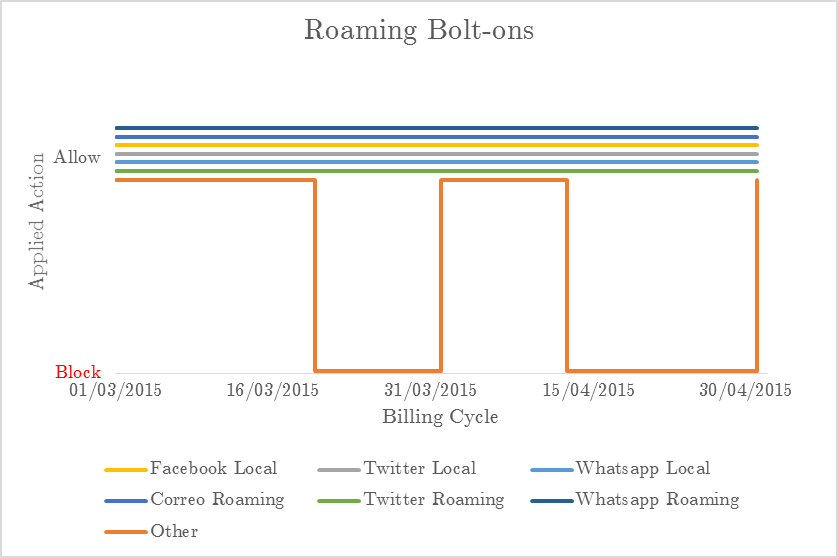
\includegraphics[width=1.00\textwidth]{image/Plans_RoamingRules}
\caption{Roaming Rules - Linear Temporal Logic}
\label{roamingRules}
\end{figure}

Figure \ref{roamingRules} above, represent the Model shown in Listing \ref{RoamingRules_Listing}. As it is, local traffic of Facebook, Twitter and Whatapp applications would always be allowed. Additionally, roaming traffic of Email, Twitter and Whatsapp applications would always be allowed too. The rest of the traffic would have being allowed and then eventually would have being blocked, when the quota is reached.  \\

The model in Listing \ref{RoamingRules_Listing}, as it is, has a flaw. Other roaming traffic would eventually consume usage from the rule[0]. This is a problem for the subscribers, as they generally cannot control which applications should be allowed and which should not from the mobile devices. That is, background applications running on their mobiles, would consume their main usage while they are on roaming without subscribers even noticing it. To solve this flaw, one additional rule needs to be considered, as shown in Listing \ref{RoamingRules2_Listing} below. \\ 

\singlespacing
\begin{lstlisting}[caption=Core-Rules-based Roaming Plan Model - II,
  label=RoamingRules2_Listing]
   ...
   
   // Unlimited Email Roaming Bolt-on
   Rules[4].conditions.application = 3;
   Rules[4].conditions.location = 1;
   Rules[4].action.underquota = 1;
   Rules[4].action.overquota = 1;
   Rules[4].p = 2;

   // Unlimited Twitter Roaming Bolt-on
   Rules[5].conditions.application = 1;
   Rules[5].conditions.location = 1;
   Rules[5].action.underquota = 1;
   Rules[5].action.overquota = 1;
   Rules[5].p = 2;

   // Unlimited Whatsapp Roaming Bolt-on
   Rules[6].conditions.application = 2;
   Rules[6].conditions.location = 1;
   Rules[6].action.underquota = 1;
   Rules[6].action.overquota = 1;
   Rules[6].p = 2;
   
   // Block other Roaming
   Rules[7].conditions.application = 255;
   Rules[7].conditions.location = 1;
   Rules[7].action.underquota = 0;
   Rules[7].action.overquota = 0;
   Rules[7].p = 1;

\end{lstlisting}
\doublespacing

Rule[7] was added in order to block always the traffic from the roaming location, specified as location 1. Note that in order to meet the desired behavior, rules [4], [5] and [6] require a higher priority than the priority of the rule [7]. When this model is verified, the priorities of the rule [7] will be updated, to show that model allow to detect that kind of wrong priority specification.\\

Figure \ref{roamingRules2} below, represent the expected behavior of this rule-based plan described previously in Listing \ref{RoamingRules_Listing} and \ref{RoamingRules2_Listing}. Note that other Roaming traffic shall always be blocked. \\

\begin{figure}[H]
\centering
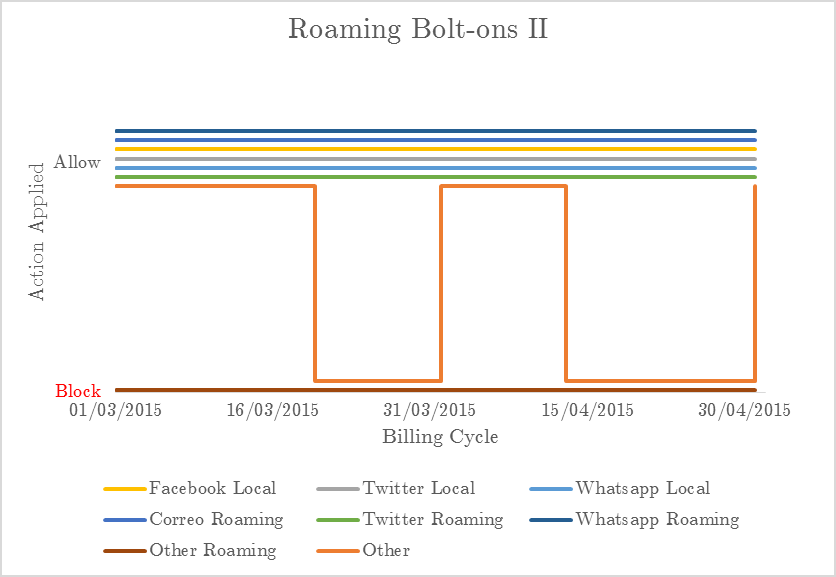
\includegraphics[width=1.00\textwidth]{image/Plans_RoamingRules2}
\caption{Roaming Rules - Linear Temporal Logic II}
\label{roamingRules2}
\end{figure}

In order to verify the expected behavior expressed above, the LTL below will be used. As seen in chapter 3, Linear-Temporal-Logic formulas are used to prove the property desired. 

\singlespacing
\begin{lstlisting}[caption=Roaming-Rules LTL,
  label=RoamingLTL]
  ltl Romaing_Rules_LTL {
    []( 
        ((generated_rule_0 -> allowed_rule_0) -> <>blocked_rule_0) &&
        (generated_rule_1->allowed_rule_1) &&
        (generated_rule_2->allowed_rule_2) &&
        (generated_rule_3->allowed_rule_3) &&
        (generated_rule_4->allowed_rule_4) &&
        (generated_rule_5->allowed_rule_5) &&
        (generated_rule_6->allowed_rule_6) &&
        (generated_rule_7->blocked_rule_7)
      )
  }
\end{lstlisting}
\doublespacing

Listing \ref{RoamingLTL} above can be translated to natural language as \emph{every} time traffic that meets the conditions of rules number 1 to 6 is generated, then it will be allowed. Additionally, \emph{every} time traffic that meets rule number 7 is generated, it will be blocked. Finally, \emph{every} time traffic that meets the condition of rule number 0 is generated, then it will be allowed and \emph{eventually} will be blocked. 

\subsection{SPIN Verification}
\noindent 
At this point we have intuitively specified the roaming rule-based plan with our Promela model (Listing \ref{RoamingRules_Listing} and \ref{RoamingRules2_Listing} above) and we have determined which LTL formulas will be used to verify the model (Listing \ref{RoamingLTL} above). Below it is presented the result obtained in Spin, with 0 errors shown in line 7.

\singlespacing
\begin{lstlisting}[caption=Core-Rules Plan Verification,
  label=RoamingResult]
(Spin Version 6.3.2 -- 17 May 2014) + Partial Order Reduction
Full statespace search for:
	never claim         	+ (Romaing_Rules_LTL)
	assertion violations	+ (if within scope of claim)
	acceptance   cycles 	+ (fairness enabled)
	invalid end states	- (disabled by never claim)
State-vector 612 byte, depth reached 94, *** errors: 0 ***
     2924 states, stored (3106 visited)
     1299 states, matched
     4405 transitions (= visited+matched)
     3703 atomic steps
hash conflicts:         0 (resolved)
Stats on memory usage (in Megabytes):
    1.751	equivalent memory usage for states (stored*(State-vector + overhead))
    1.800	actual memory usage for states
   64.000	memory used for hash table (-w24)
    0.069	memory used for DFS stack (-m2000)
   65.855	total actual memory usage
\end{lstlisting}
\doublespacing

The memory used is also relevant to note. In this test execution, the number of rules was doubled from 4 to 8. The memory required for verifying the model increased in 1.66Mb, from 64.195 Mb to 65.855 Mb. The memory used is found in the last line of each execution.

\subsubsection{Exceptions Verification}
\noindent The results obtained previously were expected as the right priorities were assigned to verify the model. Empirical tests are performed below to validate invalid models, with wrong priorities assigned. 

\singlespacing
\begin{lstlisting}[caption=Increased priority of the Roaming Rule,
  label=RoamingRules_wrong]
   ...
   // Unlimited Whatsapp Roaming Bolt-on
   Rules[6].conditions.application = 2;
   Rules[6].conditions.location = 1;
   Rules[6].action.underquota = 1;
   Rules[6].action.overquota = 1;
   Rules[6].p = 2;
   
   // Block other Roaming
   Rules[7].conditions.application = 255;
   Rules[7].conditions.location = 1;
   Rules[7].action.underquota = 0;
   Rules[7].action.overquota = 0;
   Rules[7].p = 3;

\end{lstlisting}
\doublespacing \bigskip

In the updated model above, the priority of roaming rule[7] was increased from 1 to 3. The action of the rule[7], is to block all the roaming traffic. With that priority, the other roaming applications that are supposed to be always allowed, will eventually be blocked, and consequently the model will not meet the LTL specification. That is, the rules [4], [5] and [6] will not be executed, all the roaming traffic will be handled by the rule 7, which has a higher priority assigned. SPIN model basically identifies that when whatsapp roaming traffic is generated, it is not always allowed. \\

As seen in Listing \ref{InvalidRoamingResult} below, an error is shown by the SPIN model checker. Also note that the number of states reached by the Model Checker is usually much lower when an error is found, as SPIN stops the state exploration as soon as an error is found. \\

\singlespacing
\begin{lstlisting}[caption=Invalid Roaming-Rules Plan - Verification ,
  label=InvalidRoamingResult]
(Spin Version 6.3.2 -- 17 May 2014) + Partial Order Reduction
Warning: Search not completed
Full statespace search for:
	never claim         	+ (Romaing_Rules_LTL)
	assertion violations	+ (if within scope of claim)
	acceptance   cycles 	+ (fairness enabled)
	invalid end states	- (disabled by never claim)
State-vector 612 byte, depth reached 88, *** errors: 1 ***
     1861 states, stored (2043 visited)
      865 states, matched
     2908 transitions (= visited+matched)
     2348 atomic steps
hash conflicts:         0 (resolved)
Stats on memory usage (in Megabytes):
    1.115	equivalent memory usage for states (stored*(State-vector + overhead))
    1.213	actual memory usage for states
   64.000	memory used for hash table (-w24)
    0.069	memory used for DFS stack (-m2000)
   65.270	total actual memory usage
\end{lstlisting}
\doublespacing

Another way for finding an error is having the right Model but using the wrong properties to verify it. Listing \ref{InvalidRoamingResult2} below shows the result of verifying the original Roaming Model found in Listing \ref{RoamingRules_Listing} and \ref{RoamingRules2_Listing}, with the invalid LTL below. \\

\singlespacing
\begin{lstlisting}[caption=Roaming-Rules LTL Invalidad,
  label=RoamingLTL]
  ltl Romaing_Rules_LTL_Invalid {
    []( 
        ((generated_rule_0 -> allowed_rule_0) -> <>blocked_rule_0) &&
        (generated_rule_1->allowed_rule_1) &&
        (generated_rule_2->allowed_rule_2) &&
        (generated_rule_3->allowed_rule_3) &&
        (generated_rule_4->allowed_rule_4) &&
        (generated_rule_5->allowed_rule_5) &&
        (generated_rule_6->allowed_rule_6) &&
        (generated_rule_7->allowed_rule_7)
      )
  }
\end{lstlisting}
\doublespacing

The LTL expression in line 10 above, was changed. Now the roaming traffic is expected to be always allowed. Since that is not the case, an error is shown per the output below. 

\singlespacing
\begin{lstlisting}[caption=Invalid Roaming-Rules Plan - Verification II,
  label=InvalidRoamingResult2]
(Spin Version 6.3.2 -- 17 May 2014) + Partial Order Reduction
Warning: Search not completed
Full statespace search for:
	never claim         	+ (Romaing_Rules_LTL_Invalid)
	assertion violations	+ (if within scope of claim)
	acceptance   cycles 	+ (fairness enabled)
	invalid end states	- (disabled by never claim)
State-vector 616 byte, depth reached 93, *** errors: 1 ***
     2592 states, stored (2774 visited)
     1163 states, matched
     3937 transitions (= visited+matched)
     3283 atomic steps
hash conflicts:         0 (resolved)
Stats on memory usage (in Megabytes):
    1.562	equivalent memory usage for states (stored*(State-vector + overhead))
    1.596	actual memory usage for states
   64.000	memory used for hash table (-w24)
    0.069	memory used for DFS stack (-m2000)
   65.660	total actual memory usage
\end{lstlisting}
\doublespacing

\section{Family Rules}
\subsection{Promela Model}
\noindent
Below is presented three Promela models, which represent let us represent the plan model of each family member.   

\subsubsection{Family Member \#1}
\noindent
The family plan specified in the Model below, can be used by a Family member, who wants to prevent its Smartphone to consume HD streaming videos. It consists on the Family Rule specified as the Rule[0], which is shared by all the family members, and two additional Familiy Bolt-ons rules to allow unlimited social networks (Rule [1]) and always block Streaming HD videos (Rule [2]). \\

\singlespacing
\begin{lstlisting}[caption=Family Member\#1 Model,
  label=FamilyP1_Listing]
   // Family Rule
   Rules[0].conditions.application = 255;
   Rules[0].conditions.location = 255;
   Rules[0].action.underquota = 1;
   Rules[0].action.overquota = 0;
   Rules[0].p = 0;

   // Unlimited Social Networks
   Rules[1].conditions.application = 2; // Social Networks
   Rules[1].conditions.sub_application = 255; // All Social Networks
   Rules[1].conditions.location = 0;
   Rules[1].action.underquota = 1;
   Rules[1].action.overquota = 1;
   Rules[1].p = 1;

   // HD Blocked
   Rules[2].conditions.application = 1; // Video Streaming
   Rules[2].conditions.sub_application = 1; // Only HD Streaming
   Rules[2].conditions.location = 0;
   Rules[2].action.underquota = 0;
   Rules[2].action.overquota = 0;
   Rules[2].p = 1;
\end{lstlisting}
\doublespacing

\subsubsection{Family Member \#2}
\noindent
The family plan specified in the Model below, can be used by a Family member, who wants to have blocked Social Networks and HD Streaming Videos traffic. It consists of the same Family Rule specified as the Rule[0], shared by all the family members, and two additional Familiy Bolt-ons rules to always block social networks (Rule [1]) and always block Streaming HD videos (Rule [2]). \\

\singlespacing
\begin{lstlisting}[caption=Family Member\#2 Model,
  label=FamilyP2_Listing]
   // Family Rule
   Rules[0].conditions.application = 255;
   Rules[0].conditions.location = 255;
   Rules[0].action.underquota = 1;
   Rules[0].action.overquota = 0;
   Rules[0].p = 0;

   // Blocked Social Networks
   Rules[1].conditions.application = 2; // Social Networks
   Rules[1].conditions.sub_application = 255; // All Social Networks
   Rules[1].conditions.location = 0;
   Rules[1].action.underquota = 0;
   Rules[1].action.overquota = 0;
   Rules[1].p = 1;

   // HD Blocked
   Rules[2].conditions.application = 1; // Video Streaming
   Rules[2].conditions.sub_application = 1; // Only HD Streaming
   Rules[2].conditions.location = 0;
   Rules[2].action.underquota = 0;
   Rules[2].action.overquota = 0;
   Rules[2].p = 1;
\end{lstlisting}
\doublespacing

\subsubsection{Family Member \#3}
\noindent
The family plan specified in the Model below, can be used by a Family member, who wants to have an optimized experience in Streaming Videos. It consists of the same Family Rule specified as the Rule[0], shared by all the family members, and one additional rule to optimize Streaming Video (Rule [1]). \\

\singlespacing
\begin{lstlisting}[caption=Family Member\#3 Model,
  label=FamilyP2_Listing]
   // Family Rule
   Rules[0].conditions.application = 255;
   Rules[0].conditions.location = 255;
   Rules[0].action.underquota = 1;
   Rules[0].action.overquota = 0;
   Rules[0].p = 0;

   // Optimize Streaming Video
   Rules[1].conditions.application = 1; // Video Streaming
   Rules[1].conditions.sub_application = 255; // All Video Streaming
   Rules[1].conditions.location = 0;
   Rules[1].action.underquota = 1;
   Rules[1].action.overquota = 1;
   Rules[1].p = 1;
\end{lstlisting}
\doublespacing


\subsection{System Properties}
\noindent The key rule of all the family plans above, is the Rule[0]; it dictates how most of the traffic should be handled by a shared quota. As before, we are specifying no condition for that rule and indicating to apply the block action when the quota is reached.  \\

Additionally, each plan includes different bolt-on rules, to either allow or block certain applications. \\

In order to verify the expected behavior of each Family-member plan, the following LTL formulas will be used. As previously studied, Linear-Temporal-Logic formulas are used to prove the desired properties. In this case, no new property is being used to verify this Family Plan composed by three family members.  \\

\singlespacing
\begin{lstlisting}[caption=Family Member\#1 LTL,
  label=Family1LTL]
  ltl ltl_family_member_N1 {
    []( 
        ((generated_rule_0 -> allowed_rule_0) -> <>blocked_rule_0) &&
        (generated_rule_1->allowed_rule_1) &&
        (generated_rule_2->blocked_rule_2) 
      ) 
  }
\end{lstlisting}
\doublespacing

\singlespacing
\begin{lstlisting}[caption=Family Member\#2 LTL,
  label=Family2LTL]
  ltl ltl_family_member_N2 {
    []( 
        ((generated_rule_0 -> allowed_rule_0) -> <>blocked_rule_0) &&
        (generated_rule_1->blocked_rule_1) &&
        (generated_rule_2->blocked_rule_2) 
      ) 
  }
\end{lstlisting}
\doublespacing

\singlespacing
\begin{lstlisting}[caption=Family Member\#3 LTL,
  label=Family3LTL]
  ltl ltl_family_member_N3 {
    []( 
        ((generated_rule_0 -> allowed_rule_0) -> <>blocked_rule_0) &&
        (generated_rule_1->allowed_rule_1)
      )
  }
\end{lstlisting}
\doublespacing

\subsection{SPIN Verification}
\noindent 
Listings \ref{Family1Result}, \ref{Family2Result} and \ref{Family3Result} below, presents the result obtained in Spin. Per the previous results obtained, it is clear that no error will be shown. 

\singlespacing
\begin{lstlisting}[caption=Family Member\#1 Plan Verification,
  label=Family1Result]
(Spin Version 6.3.2 -- 17 May 2014) + Partial Order Reduction
Full statespace search for:
	never claim         	+ (ltl_family_member_N1)
	assertion violations	+ (if within scope of claim)
	acceptance   cycles 	+ (fairness enabled)
	invalid end states	- (disabled by never claim)
State-vector 252 byte, depth reached 54, *** errors: 0 ***
      259 states, stored (316 visited)
      109 states, matched
      425 transitions (= visited+matched)
      261 atomic steps
hash conflicts:         0 (resolved)
Stats on memory usage (in Megabytes):
    0.066	equivalent memory usage for states (stored*(State-vector + overhead))
    0.144	actual memory usage for states
   64.000	memory used for hash table (-w24)
    0.069	memory used for DFS stack (-m2000)
   64.195	total actual memory usage
\end{lstlisting}
\doublespacing

\singlespacing
\begin{lstlisting}[caption=Family Member\#2 Plan Verification,
  label=Family2Result]
(Spin Version 6.3.2 -- 17 May 2014) + Partial Order Reduction
Full statespace search for:
	never claim         	+ (ltl_family_member_N2)
	assertion violations	+ (if within scope of claim)
	acceptance   cycles 	+ (fairness enabled)
	invalid end states	- (disabled by never claim)
State-vector 252 byte, depth reached 54, *** errors: 0 ***
      259 states, stored (316 visited)
      109 states, matched
      425 transitions (= visited+matched)
      261 atomic steps
hash conflicts:         0 (resolved)
Stats on memory usage (in Megabytes):
    0.066	equivalent memory usage for states (stored*(State-vector + overhead))
    0.144	actual memory usage for states
   64.000	memory used for hash table (-w24)
    0.069	memory used for DFS stack (-m2000)
   64.195	total actual memory usage
\end{lstlisting}
\doublespacing

\singlespacing
\begin{lstlisting}[caption=Family Member\#3 Plan Verification,
  label=Family3Result]
(Spin Version 6.3.2 -- 17 May 2014) + Partial Order Reduction
Full statespace search for:
	never claim         	+ (ltl_family_member_N3)
	assertion violations	+ (if within scope of claim)
	acceptance   cycles 	+ (fairness enabled)
	invalid end states	- (disabled by never claim)
State-vector 180 byte, depth reached 46, *** errors: 0 ***
      105 states, stored (137 visited)
       42 states, matched
      179 transitions (= visited+matched)
       84 atomic steps
hash conflicts:         0 (resolved)
Stats on memory usage (in Megabytes):
    0.020	equivalent memory usage for states (stored*(State-vector + overhead))
    0.144	actual memory usage for states
   64.000	memory used for hash table (-w24)
    0.069	memory used for DFS stack (-m2000)
   64.195	total actual memory usage
\end{lstlisting}
\doublespacing

\subsubsection{Exceptions Verification}
\label{sec:mutualExclusion}
\noindent The results obtained previously were expected as the right priorities were assigned to verify the model. Empirical tests are performed below to validate invalid model specifications. \\

If by any chance, the rule[1] of the Family Member \#2 plan shown in Listing \ref{FamilyP2_Listing} (Block Social Networks), were added to the Family Member \#1 plan; an error would be shown regardless the priorities assigned to this new rule. \\

An error will be always shown regardless the priorities assigned to the rules [1] of the Family Member \#1 and \#2 plans, is due the conditions of the two rules are the same. That is, they can't coexist without overriding one of them. 

\singlespacing
\begin{lstlisting}[caption=Invalidad Family Member\#1 Model,
  label=FamilyP1_Listing_error]
   // Family Rule
   Rules[0].conditions.application = 255;
   Rules[0].conditions.location = 255;
   Rules[0].action.underquota = 1;
   Rules[0].action.overquota = 0;
   Rules[0].p = 0;

   // Unlimited Social Networks
   Rules[1].conditions.application = 2; // Social Networks
   Rules[1].conditions.sub_application = 255; // All Social Networks
   Rules[1].conditions.location = 0;
   Rules[1].action.underquota = 1;
   Rules[1].action.overquota = 1;
   Rules[1].p = 2;

   // HD Blocked
   Rules[2].conditions.application = 1; // Video Streaming
   Rules[2].conditions.sub_application = 1; // Only HD Streaming
   Rules[2].conditions.location = 0;
   Rules[2].action.underquota = 0;
   Rules[2].action.overquota = 0;
   Rules[2].p = 2;
   
   // Blocked Social Networks
   Rules[3].conditions.application = 2; // Social Networks
   Rules[3].conditions.sub_application = 255; // All Social Networks
   Rules[3].conditions.location = 0;
   Rules[3].action.underquota = 0;
   Rules[3].action.overquota = 0;
   Rules[3].p = [1,2,3];
   
\end{lstlisting}
\doublespacing

Regardless the priority assigned to Rule[3] above (e.g. 1, 2 or 3), the following error is shown as the rules [1] and [3] cannot coexist in the same plan:\\

 \singlespacing
\begin{lstlisting}[caption=Invalidad Family Member\#1 Plan Verification,
  label=Family1Result_error]
(Spin Version 6.3.2 -- 17 May 2014) + Partial Order Reduction
Warning: Search not completed
Full statespace search for:
	never claim         	+ (ltl_family_member_N1_invalid)
	assertion violations	+ (if within scope of claim)
	acceptance   cycles 	+ (fairness enabled)
	invalid end states	- (disabled by never claim)
State-vector 328 byte, depth reached 62, *** errors: 1 ***
      435 states, stored (517 visited)
      190 states, matched
      707 transitions (= visited+matched)
      488 atomic steps
hash conflicts:         0 (resolved)
Stats on memory usage (in Megabytes):
    0.143	equivalent memory usage for states (stored*(State-vector + overhead))
    0.241	actual memory usage for states
   64.000	memory used for hash table (-w24)
    0.069	memory used for DFS stack (-m2000)
   64.293	total actual memory usage
\end{lstlisting}
\doublespacing

The issue of two rules with exact the same conditions is addressed below, in the section ``Limited Bolt-on Rules'' of this chapter, by using a different LTL formula. 

\section{Parental-Control Rules}
\subsection{Promela Model}
\noindent
The model of the Parental-Control Rules is shown in Listing \ref{PC_Listing}. Given that a plan could consist of one or more rule instances, the worst case scenario was modeled; that is, one instance of each rule was selected to form the plan below; including one from the Core Rules.  \\

The main difference with this model, is that it requires time conditions; specified through the time\_of\_day (tod) typedef. \\

\singlespacing
\begin{lstlisting}[caption=Parental-Control-Rules-based Plan Model,
  label=PC_Listing]
   // CoreRule
   Rules[0].conditions.application = 255;
   Rules[0].conditions.location = 255;
   Rules[0].action.underquota = 1;
   Rules[0].action.overquota = 0;
   Rules[0].p = 1;

   // Block Social Networks
   Rules[1].conditions.application = 1;
   Rules[1].conditions.location = 255;
   Rules[1].conditions.tod._active = true;
   Rules[1].conditions.tod.mon.start_time = 8;
   Rules[1].conditions.tod.mon.end_time = 18;
   Rules[1].conditions.tod.mon._active = true;
   Rules[1].conditions.tod.tue.start_time = 8;
   Rules[1].conditions.tod.tue.end_time = 18;
   Rules[1].conditions.tod.tue._active = true;
   Rules[1].conditions.tod.wed.start_time = 8;
   Rules[1].conditions.tod.wed.end_time = 18;
   Rules[1].conditions.tod.wed._active = true;
   Rules[1].conditions.tod.thr.start_time = 8;
   Rules[1].conditions.tod.thr.end_time = 18;
   Rules[1].conditions.tod.thr._active = true;
   Rules[1].conditions.tod.fri.start_time = 8;
   Rules[1].conditions.tod.fri.end_time = 18;
   Rules[1].conditions.tod.fri._active = true;
   Rules[1].action.underquota = 0;
   Rules[1].action.overquota = 0;
   Rules[1].p = 2;

   // Block Gaming
   Rules[2].conditions.application = 2;
   Rules[2].conditions.location = 255;
   Rules[2].conditions.tod._active = true;
   Rules[2].conditions.tod.mon.start_time = 8;
   Rules[2].conditions.tod.mon.end_time = 18;
   Rules[2].conditions.tod.mon._active = true;
   Rules[2].conditions.tod.tue.start_time = 8;
   Rules[2].conditions.tod.tue.end_time = 18;
   Rules[2].conditions.tod.tue._active = true;
   Rules[2].conditions.tod.wed.start_time = 8;
   Rules[2].conditions.tod.wed.end_time = 18;
   Rules[2].conditions.tod.wed._active = true;
   Rules[2].conditions.tod.thr.start_time = 8;
   Rules[2].conditions.tod.thr.end_time = 18;
   Rules[2].conditions.tod.thr._active = true;
   Rules[2].conditions.tod.fri.start_time = 8;
   Rules[2].conditions.tod.fri.end_time = 18;
   Rules[2].conditions.tod.fri._active = true;
   Rules[2].action.underquota = 0;
   Rules[2].action.overquota = 0;
   Rules[2].p = 2;
   
   // Block Streaming
   Rules[3].conditions.application = 4;
   Rules[3].conditions.location = 255;
   Rules[3].action.underquota = 0;
   Rules[3].action.overquota = 0;
   Rules[3].p = 2;
   
\end{lstlisting}
\doublespacing

   
\subsection{System Properties}
\label{sec:mutualExclusion2}
\noindent The System Properties to be verified are quite similar to the previous ones used, where rule[0] has no condition so all the traffic is eventually blocked when the quota is reached. Additionally there are three more rules, each one to always block a different application when the rule conditions, including the time conditions, are met.\\

As it has been discussed, the rules mutually exclusive among themselves requires a higher priority. If any of these rules has a lower priority assigned, the Rule[0] will take precedence over that rule and consequently, the desired behavior of blocking that particular application will not be met. \\

\singlespacing
\begin{lstlisting}[caption=Parental-Control-Rules LTL,
  label=parentalControlLTL]
  ltl parental_control_LTL {
    []( 
        ((generated_rule_0 -> allowed_rule_0) -> <>blocked_rule_0) && 
        (generated_rule_1->blocked_rule_1) &&
        (generated_rule_2->blocked_rule_2) &&
        (generated_rule_3->blocked_rule_3)
      )
  }
\end{lstlisting}
\doublespacing

Listing \ref{parentalControlLTL} above can be translated to natural language as \emph{every} time traffic that meets the conditions of rule [0] is generated, then it will be allowed and \emph{eventually} will be blocked. Additionally, \emph{every} time traffic that meets rules [1], [2] and [3] is generated, it will be blocked. 

\subsection{SPIN Verification}
\noindent 
Below it is presented the result obtained in Spin, with 0 errors shown in line 7.

\singlespacing
\begin{lstlisting}[caption=Parental-Control-Rules Plan Verification,
  label=ParentalControlResult]
(Spin Version 6.3.2 -- 17 May 2014) + Partial Order Reduction
Full statespace search for:
	never claim         	+ (parental_control_LTL)
	assertion violations	+ (if within scope of claim)
	acceptance   cycles 	+ (fairness enabled)
	invalid end states	- (disabled by never claim)
State-vector 324 byte, depth reached 62, *** errors: 0 ***
      504 states, stored (586 visited)
      217 states, matched
      803 transitions (= visited+matched)
      556 atomic steps
hash conflicts:         0 (resolved)
Stats on memory usage (in Megabytes):
    0.163	equivalent memory usage for states (stored*(State-vector + overhead))
    0.241	actual memory usage for states
   64.000	memory used for hash table (-w24)
    0.069	memory used for DFS stack (-m2000)
   64.293	total actual memory usage
\end{lstlisting}
\doublespacing

\section{Limited Bolt-on Rules}
\subsection{Promela Model}
\noindent
LADD01 and LADD04 Limited Bolt-on rules were selected from Table \ref{limited_rules} above, and were combined with the unlimited bolt-on Rules seen previously to form a plan.  

\singlespacing
\begin{lstlisting}[caption=Core-Rules-based Plan Model,
  label=CoreRules_Listing]
   // CoreRule
   Rules[0].conditions.application = 255;
   Rules[0].conditions.location = 255;
   Rules[0].action.underquota = 1; //Allow Traffic
   Rules[0].action.overquota = 0; //Block Traffic
   Rules[0].p = 0; 
   
   // Unlimited local Facebook Bolt-on
   Rules[1].conditions.application = 0;
   Rules[1].conditions.location = 0;
   Rules[1].action.underquota = 1; //Allow Traffic
   Rules[1].action.overquota = 1; //Allow Traffic
   Rules[1].p = 3;

   // Unlimited local Twitter Bolt-on
   Rules[2].conditions.application = 1;
   Rules[2].conditions.location = 0;
   Rules[2].action.underquota = 1; //Allow Traffic
   Rules[2].action.overquota = 1; //Allow Traffic
   Rules[2].p = 3;

   // Unlimited local Whatsapp Bolt-on
   Rules[3].conditions.application = 2;
   Rules[3].conditions.location = 0;
   Rules[3].action.underquota = 1; //Allow Traffic
   Rules[3].action.overquota = 1; //Allow Traffic
   Rules[3].p = 3;

   // 1GB Video Streaming Optimized
   Rules[4].conditions.application = 5;
   Rules[4].conditions.location = 0;
   Rules[4].action.underquota = 1; //Allow Traffic
   Rules[4].is_uninstallable = true;
   Rules[4].p = 2;

   // 1GB Extra
   Rules[5].conditions.application = 255;
   Rules[5].conditions.location = 255;
   Rules[5].action.underquota = 1; //Allow Traffic
   Rules[5].is_uninstallable = true;
   Rules[5].p = 1;
   \end{lstlisting}
\doublespacing

Limited Bolt-on rules are specified in Rules [4] and [5] above. Rule[4] optimize Video Streaming; while Rule[5] add more volume to a Plan, for a one-time-usage. 

\subsection{System Properties}
\noindent The new LTL formulas to verify the properties of Rules [4] and [5] are shown below: 

\singlespacing
\begin{lstlisting}[caption=Limited Bolt-on Rules LTL,
  label=limitedLTL]
  ltl limitedLTL {
   []( 
      (generated_rule_1->allowed_rule_1) &&
      (generated_rule_2->allowed_rule_2) &&
      (generated_rule_3->allowed_rule_3)
     ) &&
   ([](((generated_rule_4 -> allowed_rule_4)) U overquota_rule_4)) &&
   ([](((generated_rule_5 -> allowed_rule_5)) U overquota_rule_5)) &&
   ([](((generated_rule_0 -> allowed_rule_0) -> 
         blocked_rule_0)) U (!overquota_rule_5))
  }
\end{lstlisting}
\doublespacing

Lines 2 to 6 verify the expected behavior of the rules studied previously. From line 7, a new operator is used: Until (U). Line 7 can be translated to natural language as \emph{every} time traffic that meets the conditions of rule [4] is generated, then it will be allowed until rule [4] reaches its quota. Similarly, Line 8, as \emph{every} time traffic that meets the conditions of rule [5] is generated, then it will be allowed until rule [5] reaches its quota. Consequently, line 9 is translated to \emph{every} time traffic that meets the condition of rule [0] is generated, then it will be allowed and \emph{eventually} will be blocked until rule [5] is not overquota. \\

Given that Rule[0] and Rule[5] are mutually exclusive rules, the until operator in line 10 is required. As seen before in \ref{sec:mutualExclusion} and \ref{sec:mutualExclusion2}, rules that have exactly the same conditions, cannot coexist in a plan. However, the until operator above, let mutually exclusive rules coexist, only if one of the rules is temporary applied (e.g. when the quota is reached). That is, with the Until operator (U), which rule is applied is controlled. \\

\subsection{SPIN Verification}
\noindent 
We have specified a rule-based plan with a number of unlimited and limited bolt-on rules and introduced the LTL to be used to verify the Promela model of the plan.  Listing \ref{LimitedResult} below, shows no error in line 7. \\

\singlespacing
\begin{lstlisting}[caption=Limited Bolt-on-Rules Plan Verification,
  label=LimitedResult]
(Spin Version 6.3.2 -- 17 May 2014) + Partial Order Reduction
Full statespace search for:
	never claim         	+ (limitedLTL)
	assertion violations	+ (if within scope of claim)
	acceptance   cycles 	+ (fairness enabled)
	invalid end states	- (disabled by never claim)
State-vector 468 byte, depth reached 76, *** errors: 0 ***
     3725 states, stored (13883 visited)
    12596 states, matched
    26479 transitions (= visited+matched)
    24133 atomic steps
hash conflicts:         0 (resolved)
Stats on memory usage (in Megabytes):
    1.719	equivalent memory usage for states (stored*(State-vector + overhead))
    1.796	actual memory usage for states
   64.000	memory used for hash table (-w24)
    0.069	memory used for DFS stack (-m2000)
   65.855	total actual memory usage
\end{lstlisting}
\doublespacing

\subsubsection{Exceptions Verification}
\noindent No error was shown in Listing \ref{LimitedResult} above, as the Until operator (U) was used. If a different LTL formula, with no Until operator, were used to verify the Model, as below, an error would be shown by Spin Model Checker. The invalid LTL is presented in Listing \ref{InvalidlimitedLTL} below, where no Until operator is used and the corresponding result is presented in Listing \ref{InvalidLimitedResult}.   \\

\singlespacing
\begin{lstlisting}[caption=Invalid Limited Bolt-on Rules LTL,
  label=InvalidlimitedLTL]
  ltl InvalidLimitedLTL {
   []( 
      (generated_rule_1->allowed_rule_1) &&
      (generated_rule_2->allowed_rule_2) &&
      (generated_rule_3->allowed_rule_3)
     ) &&
   ([](((generated_rule_4 -> allowed_rule_4)))) &&
   ([](((generated_rule_5 -> allowed_rule_5)))) &&
   ([](((generated_rule_0 -> allowed_rule_0) -> 
         blocked_rule_0)))
  }
\end{lstlisting}
\doublespacing

\singlespacing
\begin{lstlisting}[caption=Invalid Limited Bolt-on-Rules Plan Verification,
  label=InvalidLimitedResult]
(Spin Version 6.3.2 -- 17 May 2014) + Partial Order Reduction
Warning: Search not completed
Full statespace search for:
	never claim         	+ (InvalidlimitedLTL)
	assertion violations	+ (if within scope of claim)
	acceptance   cycles 	+ (fairness enabled)
	invalid end states	- (disabled by never claim)
State-vector 468 byte, depth reached 58, *** errors: 1 ***
       59 states, stored
       13 states, matched
       72 transitions (= stored+matched)
       33 atomic steps
hash conflicts:         0 (resolved)
Stats on memory usage (in Megabytes):
    0.027	equivalent memory usage for states (stored*(State-vector + overhead))
    0.143	actual memory usage for states
   64.000	memory used for hash table (-w24)
    0.069	memory used for DFS stack (-m2000)
   64.195	total actual memory usage
\end{lstlisting}
\doublespacing

\section{Result Analysis and Discussion}
\noindent
The main highlights of each verified use-case scenario is summarized in table \ref{results} below. Additionally, the maximum concurrent rules verified on each use-case, along with its memory usage and the properties used during the verification, are also detailed. 

\begin{table}[H]
\begin{center}
\scalebox{0.8}{	
\begin{tabular}{| l || p{7.6cm} | p{4cm} | l |}
\hline
\textbf{Use Case} & \textbf{Highlights} & \textbf{Concurrent Rules} & \textbf{Properties}\\
 \hline \hline
\emph{Core Rules} & 
\makecell[l]{Basic use-case is presented. \\ Always operator ($\square$) is introduced. \\ Eventually operator ($\lozenge$)  is introduced.}
& 4 Rules (64.195 MB) & PT01, PT02\\ \hline
\emph{Roaming Bolt-on Rules} & \makecell[l]{Basic use-case is extended with Roaming \\ Bolt-on rules. \\ Significance of having the right priority \\is illustrated.}
& 7 Rules (65.855 MB) & PT01, PT02\\ \hline
\emph{Family Rules} & \makecell[l]{Application and sub-application conditions \\are considered.\\An example is shown where rules with the\\ same conditions cannot co-exist with the \\LTL used so far. }
& 3 Rules (64.195 MB) & PT01, PT02\\ \hline
\emph{Parental-Control Rules} & \makecell[l]{Time-of-day conditions are considered.}
& 4 Rules (64.293 MB) & PT01, PT02\\ \hline
\emph{Limited Bolt-on Rules} & \makecell[l]{Complex use-case is presented, where \\temporary bolt-on rules are used. \\Until(U) operator is introduced.}
& 6 Rules (65.855 MB) & \makecell[l]{PT01, PT02,\\PT03, PT04}\\ \hline
\end{tabular}}
\end{center}
\caption{Summary of results}
\label{results}
\end{table}

As seen in table \ref{results} above, most of the use-cases were verified using the properties PT01 and PT02 -- that is because the \emph{Until} operator (\emph{U}) is only required when a rule needs to be applied until some other event occurs. On the other hand, Always ($\square$) and Eventually ($\lozenge$) operators were always used to verify the use-cases. \\

Each of the use-cases above, considers a different rule condition or a new property not verified before -- this, to let us illustrate the application of each condition or property. More complex plans, not covered in the use-cases above, may be modeled, specified and verified by combining the conditions used with their corresponding properties. For example, Time of Day conditions may be used with the location condition. The device condition was not used on the use-cases, but its application is similar to the other conditions (e.g. location). 

Our proposed Promela model, introduced in figure \ref{TypeDef_Diagram}, can be intuitively extended to support more conditions not considered in this thesis. \\

The memory required for verifying the use-cases was fairly low. However, as more rules are specified in a plan, more memory would be required. That is, models with many plans and rules may require huge amounts of memory -- an exponential relation between the number of rules and properties used, with the required memory is presumed. \\

\clearpage

